%% Computational Optimization and Applications -- Springer Nature template (sn-jnl).
\documentclass[pdflatex,sn-mathphys-num]{sn-jnl}

\usepackage{graphicx}
\usepackage{multirow}
\usepackage{amsmath,amssymb,amsfonts}
\usepackage{amsthm}
\usepackage{mathrsfs}
\usepackage{xcolor}
\usepackage{textcomp}
\usepackage{manyfoot}
\usepackage{booktabs}
\usepackage{algorithm}
\usepackage{algorithmicx}
\usepackage{algpseudocode}
\usepackage{url}
\usepackage{longtable}
\usepackage{array}
\newcolumntype{P}[1]{>{\raggedright\arraybackslash}p{#1}}
% Long monospaced names are not hyphenated by default.
\usepackage[htt]{hyphenat}
% Shrinks a wide table only when it would run into the margin.
\usepackage{adjustbox}
\newcommand{\fittable}[1]{\adjustbox{max width=\textwidth}{#1}}
\usepackage{tikz}
\usetikzlibrary{fit,backgrounds,arrows.meta,positioning,shapes.geometric}

\theoremstyle{thmstyleone}%
\newtheorem{theorem}{Theorem}%
\newtheorem{proposition}[theorem]{Proposition}%
\newtheorem{corollary}[theorem]{Corollary}%
\newtheorem{lemma}[theorem]{Lemma}%
\theoremstyle{thmstyletwo}%
\newtheorem{remark}{Remark}%

% sn-jnl wraps tables in threeparttable, which breaks a tabular placed inside a box;
% use the plain table environment with the class's table font instead.
\renewenvironment{table}[1][]{\begin{tableorg}[#1]\begin{center}\tablebodyfont}{\end{center}\end{tableorg}}

\raggedbottom

\begin{document}

\title[Exact large-neighbourhood search for maximum independent set]{Exact Large-Neighbourhood Search for the Maximum Independent Set Problem on Massive Sparse Graphs}

\author*[1]{\fnm{Quang-Vinh} \sur{Dang}}\email{vinh.dq4@buv.edu.vn}

\affil*[1]{\orgname{British University Vietnam}, \orgaddress{\city{Hung Yen}, \country{Vietnam}}}

\abstract{The maximum independent set problem on large sparse graphs is usually attacked by safe reduction rules followed by local search. We present Cascade, a local search built on a region move: a set $F$ of incumbent vertices is released, the outside vertices whose incumbent neighbours all lie in $F$ are collected, and the resulting region is re-solved by branch-and-reduce. Because nothing outside the region conflicts with it, the incumbent never worsens. The region construction is known from dynamic independent-set maintenance; Cascade applies it to static graphs, runs reductions inside each region, and adapts $|F|$ online without per-instance tuning. On 27 instances in five families at a 60-second budget, Cascade matches or exceeds the best of six established solvers on 16 instances, including all six geometric graphs, and is strictly best on three Delaunay triangulations. Ablations show that exact repair and reductions inside the region each contribute to solution quality, and measurements of the residual kernel show that its size alone does not predict where the move helps.}

\keywords{maximum independent set, large neighbourhood search, data reduction, kernelization, combinatorial optimization}

\maketitle

\section{Introduction}
\label{sec:intro}

Given an undirected graph $G=(V,E)$, the maximum independent set problem asks
for a largest set of pairwise non-adjacent vertices. It is equivalent to the
minimum vertex cover problem on $G$ and to maximum clique on the complement.
The problem is NP-hard and admits no constant-factor approximation unless
P${}={}$NP, so large instances are attacked heuristically. It models any
selection of a largest mutually compatible set under pairwise conflicts, for
example jobs with conflicting resources, interfering transmitters, overlapping
label placements or duplicate records, and the conflict graphs that arise from
such data routinely have millions of vertices and low average degree.

Over the last decade the practical state of the art has converged on one
template: apply \emph{safe data reduction rules} until none fires, then search
whatever survives. Solvers differ in what they do once the rules stall.
Reducing-peeling \citep{chang2017} performs one greedy descent. ReduMIS
\citep{lamm2017} and OnlineMIS \citep{dahlum2016} run swap-based local search on
the reduced graph. Branch-and-reduce \citep{akiba2016} is complete but
exponential. NuMVC \citep{cai2013numvc} and FastVC \citep{cai2017fastvc}, from the
vertex cover literature, are strong on small dense instances but lose ground on
graphs with millions of vertices. All of these are weakest where the reduced
graph, or \emph{kernel}, stays large; Delaunay triangulations are the canonical
example.

\paragraph{The idea in one example} Suppose a maximal independent set $S$ is in
hand and nothing can be added. A classical $(1,2)$-swap asks: if one vertex $v$ of
$S$ is removed, do two non-adjacent vertices become available? Those two must have
$v$ as their \emph{only} neighbour in $S$. The same question can be asked about
two or ten removed vertices at once: remove a set $F$ of solution vertices and
collect every outside vertex all of whose solution neighbours lie in $F$. These
vertices, together with $F$, form a \emph{region}; nothing outside the region
touches the solution inside it, so any independent set of the region can be swapped
in for $F$ without checking the rest of the graph. The best swap for this $F$ is
the maximum independent set of the region, a smaller instance of the same problem.
Figures~\ref{fig:region} and~\ref{fig:move} show a case where releasing one vertex
never helps and releasing several does.

This is large-neighbourhood search \citep{hashimoto2019,katzmann2017} for the
independent set problem, and the construction of the region is not new: it is the
one used by \citet{borowitz2025} in the dynamic setting, where an edge update
triggers an exactly solved local subproblem (Section~\ref{sec:related}). This paper
uses that construction as the inner move of a \emph{static} solver for massive
graphs, with reductions applied inside each region and an online rule for how many
solution vertices to release. Our contributions are:
\begin{enumerate}
\item a static region-move local search with a proof that an incumbent is never
      worsened when sub-solves are truncated (Section~\ref{sec:move}), and an
      explicit comparison with the region constructions of \citet{borowitz2025},
      \citet{hashimoto2019} and swap neighbourhoods (Table~\ref{tab:frameworks});
\item an online rule for the number of released vertices, with a stated schedule
      and a sensitivity study (Section~\ref{sec:search});
\item a dynamic graph with last-in-first-out undo that lets reductions run inside
      the move (Section~\ref{sec:implementation});
\item a computational study on 27 instances, including measurements that tie the
      method's behaviour to the residual kernel, to whether the region sub-solve is
      exact and to whether reductions run inside the region
      (Section~\ref{sec:experiments}). The positive result is narrow and we
      delimit it.
\end{enumerate}
Proofs of the standard reduction rules, per-family tables and secondary experiments
are in Online Resource 1.

\subsection{Related work}
\label{sec:related}

\paragraph{Reductions and exact solvers} The reduction approach traces to the
Nemhauser--Trotter theorem \citep{nemhauser1975} and to kernelization for vertex
cover \citep{chen2001,abukhzam2007}, with local rules from exact exponential
algorithms \citep{tarjan1977,fomin2009,xiao2013,xiao2017}.
\citet{akiba2016} showed that branch-and-reduce with the full rule set is
competitive with integer programming on real instances; \citet{hespe2019}
parallelised kernelization and characterised which families reduce well, and later
work enlarges the set of applicable rules \citep{gellner2021,figiel2022,hespe2021}.
The PACE 2019 winner \citep{pace2019,hespe2020} combines kernelization, local search,
branch-and-reduce and a maximum-clique solver \citep{li2017momc}. The weighted
variant has attracted most recent activity
\citep{lamm2019,xiaowww2021,grossmann2023,langedal2022,grossmann2024survey,grossmann2025chils}.

\paragraph{Local search} \citet{andrade2012} introduced the $(1,2)$-swap with an
$O(m)$ test, which underlies the KaMIS solvers \citep{lamm2017,dahlum2016}. NuMVC
\citep{cai2013numvc} combines edge weighting with configuration checking and is
extremely strong on dense structured instances; FastVC
\citep{cai2015,cai2017fastvc} trades some quality for the ability to run on massive
graphs, and InfVC \citep{sun2025infvc} adds inference rules and a degree-biased
perturbation, reporting gains on massive instances. We did not run InfVC
(Section~\ref{sec:threats}).

\paragraph{Neighbourhood search with exactly solved subproblems}
\citet{andrade2012} introduced $(j,k)$-swaps; \citet{hashimoto2019} extend the
$(k,\ell)$ neighbourhood to the weighted problem and embed branch-and-bound in the
local search; \citet{katzmann2017} search the $k$-swap neighbourhood of vertex cover
systematically in $\Delta^{O(k)}n$ time. The closest work is that of
\citet{borowitz2025}, who maintain an independent set under edge updates: after an
update the greedy repair cannot absorb, they build a subgraph $H$ by a bounded-depth
breadth-first search, add the incumbent neighbours of $H$ and the tight vertices of
$N(H)\setminus H$, and solve the induced subgraph with KaMIS branch-and-reduce
\citep{lamm2019}, capping $|H|$ by $\nu_{\max}$ and pruning high-degree vertices.

The region of Section~\ref{sec:move} is the same object: with $F$ the incumbent
vertices of their closed subgraph, their region is $R(F)$.
\emph{Theorem~\ref{thm:region} is therefore not a new observation}; we state and
prove it for self-containedness, and reductions on the region are likewise present
in their work through the sub-solver. Table~\ref{tab:frameworks} lists what differs:
the setting (static against dynamic), how the released set is chosen, how its size
is controlled (an online rule against a fixed cap), the absence of pruning here, and
the sub-solver (an in-house reusable branch-and-reduce engine). Whether those
differences matter on static graphs is empirical, and Section~\ref{sec:regional}
measures the parts that can be isolated within our own implementation. We did not
run their code.

\begin{table}[htbp]
\centering
\caption{Region-based neighbourhood search frameworks compared. ``Released set'' is
the set of incumbent vertices removed before the region is re-solved.}
\label{tab:frameworks}
\footnotesize
\fittable{
\begin{tabular}{P{2.3cm}P{3.0cm}P{3.0cm}P{3.0cm}P{3.0cm}}
\toprule
 & Andrade et al.~\cite{andrade2012} & Hashimoto et al.~\cite{hashimoto2019} & Borowitz et al.~\cite{borowitz2025} & This work \\
\midrule
Problem & unweighted, static & weighted, static & (weighted) dynamic & unweighted, static \\
Released set & $j\le 2$ vertices, enumerated & $k$ vertices dropped, candidates restricted & incumbent vertices met by BFS of depth $d$, closed under neighbours & $k$ incumbent vertices along a BFS walk from a seed \\
Candidate restriction & only vertices with the released set as sole solution neighbours & $(k,\ell)$ candidate lists & tight vertices of $N(H)\setminus H$; high-degree vertices pruned & all tight vertices (no pruning) \\
Objective & best $(j,k)$-swap & best $(k,\ell)$-swap & MIS of $G[H]$ & MIS of $G[R(F)]$ \\
Reductions & none & none in the move & inside KaMIS BnR & inside the move \\
Sub-solver & enumeration & branch-and-bound & KaMIS BnR, time-capped & in-house, node- and time-capped \\
Size control & fixed & fixed & fixed ($d$, $\nu_{\max}$) & online \\
\bottomrule
\end{tabular}}
\end{table}

\section{Preliminaries}
Let $G=(V,E)$ be a simple undirected graph. A set $S \subseteq V$ is
\emph{independent} if no edge has both endpoints in $S$; $\alpha(G)$ is the
maximum size of such a set. $N(v)$ is the neighbourhood of $v$ and
$N[v]=N(v)\cup\{v\}$. A rule transforming $G$ into $G'$ with an offset $c$ is
\emph{safe} if $\alpha(G)=\alpha(G')+c$ and a maximum independent set of $G$ can be
reconstructed from one of $G'$. We use the rule set that is standard in this
literature \citep{akiba2016,lamm2017,hespe2019}, in Table~\ref{tab:rules}; a graph on
which no rule fires is a \emph{kernel}. Each rule records how to reconstruct a
solution, and \emph{lifting} replays those records in reverse. Proofs of the
simplicial, domination and degree-2 folding rules are in Online Resource 1.

\begin{table}[htbp]
\centering
\caption{The reduction rules used. The unconfined rule is that of
\citet{xiao2017}; the LP rule is that of \citet{nemhauser1975}.}
\label{tab:rules}
\small
\begin{tabular}{lll}
\toprule
Rule & Condition & Effect \\
\midrule
Degree-0 & $\deg(v)=0$ & take $v$ \\
Degree-1 & $N(v)=\{u\}$ & take $v$, discard $u$ \\
Simplicial & $N(v)$ is a clique & take $v$, discard $N(v)$ \\
Degree-2 fold & $N(v)=\{u,w\}$, $uw \notin E$ & replace $v,u,w$ by one vertex \\
Twin & $N(u)=N(v)$, $|N(u)|=3$ & take both, or fold \\
Domination & $uv \in E$, $N[u] \subseteq N[v]$ & discard $v$ \\
Unconfined & confining-set test fails & discard $v$ \\
LP & half-integral LP optimum & fix the integral part \\
\bottomrule
\end{tabular}
\end{table}

\paragraph{Twin} Two non-adjacent degree-three vertices $u,v$ with the same
neighbourhood $\{p,q,r\}$ are twins. A solution that uses one of $p,q,r$ gives up
both $u$ and $v$, so only two outcomes matter: both twins are taken, or all of
$p,q,r$ are. If the neighbourhood contains an edge, at most two of $p,q,r$ can be
taken, so taking $u$ and $v$ is never worse (delete $p,q,r$). If it is independent
we \emph{fold}: replace the five vertices by one vertex $f$ adjacent to every other
neighbour of $p,q,r$ and add $2$ to the offset, so that $f$ stands for $\{p,q,r\}$
and its absence for $\{u,v\}$ \citep{akiba2016}.

\paragraph{Unconfined} Start from $S=\{v\}$. A vertex $u\in N(S)$ with exactly one
neighbour in $S$ is a \emph{child}. If some child has $N(u)\subseteq N[S]$, swapping
$S$ for $u$ in any independent set containing $v$ loses nothing, so $v$ is
discarded. If the child's remaining neighbourhood is a single vertex $w$, then $w$
is added to $S$ and the test continues; otherwise $v$ is \emph{confined}. Domination
is the case $S=\{v\}$ \citep{xiao2013,xiao2017}. We cap $|S|$ at eight and the edges
scanned per test at $2\times10^4$; a capped test answers ``confined'', so the cap
cannot make the rule unsound.

\paragraph{LP} Relax vertex cover to $x_v\in[0,1]$ with $x_u+x_v\ge 1$ on every
edge. The optimum is half-integral \citep{nemhauser1975}, and some maximum
independent set contains every vertex with $x_v=0$ and avoids every vertex with
$x_v=1$; only vertices at $\tfrac12$ remain. The optimum comes from a maximum
matching in the bipartite double cover via K\"onig's theorem. It is the only rule
that looks at the whole graph, which is why it fires where the local rules have
stalled; it must run to completion for persistency to hold, so it is skipped
rather than interrupted when the budget is short.

\begin{figure}[htbp]
\centering
\resizebox{0.8\textwidth}{!}{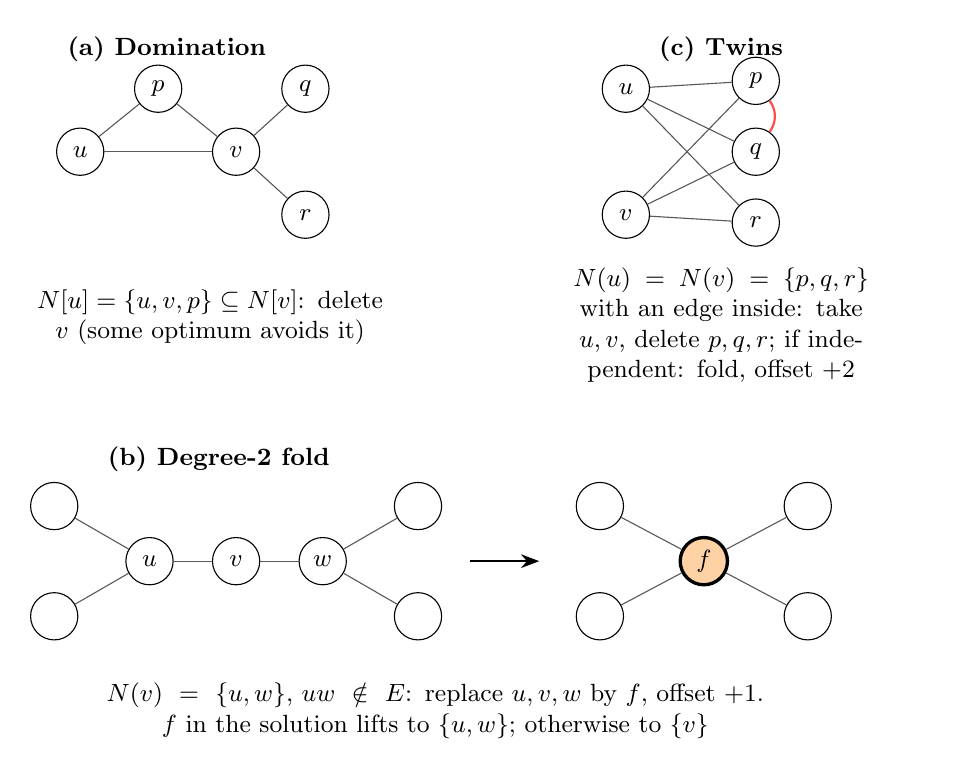
\begin{tikzpicture}[
  every node/.style={font=\small},
  vtx/.style={circle,draw,minimum size=6mm,inner sep=0pt,fill=white},
  tk/.style={vtx,fill=green!25,very thick},
  dl/.style={vtx,fill=black!12,dashed},
  fd/.style={vtx,fill=orange!35,very thick},
  ed/.style={draw,black!65},
  arr/.style={-{Stealth},thick},
  x=11mm,y=10mm]

% ---- (a) domination ----
\begin{scope}
  \node at (1.0,2.5) {\textbf{(a) Domination}};
  \node[vtx] (u) at (0,1.2) {$u$}; \node[vtx] (v) at (1.8,1.2) {$v$};
  \node[vtx] (p) at (0.9,2.0) {$p$}; \node[vtx] (q) at (2.6,2.0) {$q$}; \node[vtx] (r) at (2.6,0.4) {$r$};
  \foreach \s/\t in {u/v,u/p,v/p,v/q,v/r} \draw[ed] (\s)--(\t);
  \node[align=center,text width=4.4cm] at (1.5,-0.9) {$N[u]=\{u,v,p\}\subseteq N[v]$: delete $v$ (some optimum avoids it)};
\end{scope}

% ---- (b) degree-2 fold ----
\begin{scope}[yshift=-5.2cm]
  \node at (1.6,2.5) {\textbf{(b) Degree-2 fold}};
  \node[vtx] (x1) at (-0.3,1.9) {}; \node[vtx] (x2) at (-0.3,0.5) {};
  \node[vtx] (a) at (0.8,1.2) {$u$}; \node[vtx] (b) at (1.8,1.2) {$v$}; \node[vtx] (c) at (2.8,1.2) {$w$};
  \node[vtx] (y1) at (3.9,1.9) {}; \node[vtx] (y2) at (3.9,0.5) {};
  \foreach \s/\t in {x1/a,x2/a,a/b,b/c,c/y1,c/y2} \draw[ed] (\s)--(\t);
  \draw[arr] (4.5,1.2)--(5.3,1.2);
  \node[vtx] (x1b) at (6.0,1.9) {}; \node[vtx] (x2b) at (6.0,0.5) {};
  \node[fd] (f) at (7.2,1.2) {$f$};
  \node[vtx] (y1b) at (8.4,1.9) {}; \node[vtx] (y2b) at (8.4,0.5) {};
  \foreach \s/\t in {x1b/f,x2b/f,f/y1b,f/y2b} \draw[ed] (\s)--(\t);
  \node[align=center,text width=10cm] at (4.1,-0.7) {$N(v)=\{u,w\}$, $uw\notin E$: replace $u,v,w$ by $f$, offset $+1$.\\ $f$ in the solution lifts to $\{u,w\}$; otherwise to $\{v\}$};
\end{scope}

% ---- (c) twin ----
\begin{scope}[xshift=6.6cm]
  \node at (1.4,2.5) {\textbf{(c) Twins}};
  \node[vtx] (t1) at (0.3,2.0) {$u$}; \node[vtx] (t2) at (0.3,0.4) {$v$};
  \node[vtx] (n1) at (1.8,2.1) {$p$}; \node[vtx] (n2) at (1.8,1.2) {$q$}; \node[vtx] (n3) at (1.8,0.3) {$r$};
  \foreach \s in {n1,n2,n3} {\draw[ed] (t1)--(\s); \draw[ed] (t2)--(\s);}
  \draw[ed,thick,red!70] (n1) to[bend left=35] (n2);
  \node[align=center,text width=5cm] at (1.4,-1.0) {$N(u)=N(v)=\{p,q,r\}$ with an edge inside: take $u,v$, delete $p,q,r$; if independent: fold, offset $+2$};
\end{scope}
\end{tikzpicture}
}
\caption{Three rules on small examples. (a)~Domination deletes $v$ because $u$ is
adjacent to it and sees nothing $v$ does not. (b)~Degree-2 folding contracts the
path $u,v,w$ into one vertex $f$: choosing $f$ stands for taking both ends, not
choosing it for taking the middle vertex. (c)~Twins with an edge among the
neighbours (red): at most two of them can be used, so taking $u$ and $v$ is never
worse.}
\label{fig:rules}
\end{figure}

\section{The region move}
\label{sec:move}

Let $S$ be an independent set of $G$ and let $F \subseteq S$. Define
\begin{equation}
R(F) \;=\; F \;\cup\; \{\, u \in V \setminus S \;:\; N(u) \cap S \subseteq F \,\}.
\label{eq:region}
\end{equation}

\begin{theorem}
\label{thm:region}
With $S$, $F$ and $R(F)$ as above:
\begin{enumerate}
\item[(a)] no edge of $G$ joins $R(F)$ to $S \setminus R(F)$;
\item[(b)] for every independent set $T$ of the induced subgraph $G[R(F)]$, the
      set $(S \setminus R(F)) \cup T$ is independent in $G$;
\item[(c)] $S \cap R(F) = F$, and consequently $\alpha(G[R(F)]) \ge |F|$.
\end{enumerate}
\end{theorem}

\begin{proof}
(a) Let $v \in R(F)$ and $w \in S \setminus R(F)$ and suppose $vw \in E$. If
$v \in F$ then $v,w \in S$ are adjacent, contradicting independence of $S$.
Otherwise $v \notin S$, so $w \in N(v) \cap S \subseteq F \subseteq R(F)$,
contradicting $w \notin R(F)$.

(b) $T$ is independent, $S \setminus R(F)$ is independent as a subset of $S$,
and by (a) no edge joins the two sets.

(c) $F \subseteq S \cap R(F)$ holds by construction. Conversely, an
$x \in S \cap R(F)$ with $x \notin F$ would belong to $V \setminus S$ by
\eqref{eq:region}, a contradiction. Hence $S \cap R(F) = F$, which is an
independent set of $G[R(F)]$, so $\alpha(G[R(F)]) \ge |F|$.
\end{proof}

\begin{remark}[Attribution]
\label{rem:attr}
Part~(a) is the closure property that \citet{borowitz2025} obtain by adding the
incumbent neighbours of $H$ and the tight vertices of $N(H)\setminus H$; their
subgraph is $R(F)$ for $F$ the incumbent vertices it contains. We claim
the statements and proofs below only as a self-contained account of why the move
is admissible, not as a new construction.
\end{remark}

\begin{proposition}[Residual form]
\label{prop:residual}
$R(F) = V \setminus N[S \setminus F]$. Hence solving $G[R(F)]$ is exactly the
maximum independent set problem on the residual graph obtained by fixing
$S \setminus F$ into the solution.
\end{proposition}

\begin{proof}
A vertex $u \notin S$ lies in $R(F)$ iff $N(u)\cap S\subseteq F$ iff $u$ has no
neighbour in $S\setminus F$ iff $u \notin N[S\setminus F]$ (it is not in
$S \setminus F$ itself). A vertex $u\in S$ lies in $R(F)$ iff $u\in F$ iff
$u\notin S\setminus F$; and every vertex of $S \setminus F$ is in
$N[S\setminus F]$, while a vertex of $F$ is not adjacent to $S\setminus F$
because $S$ is independent.
\end{proof}

Proposition~\ref{prop:residual} is the framing under which the move is a
standard ``fix and optimise'' large-neighbourhood step: choose which part of the
incumbent to keep, and re-solve the rest. It also explains why the region cannot
be enlarged by hand: any vertex outside $R(F)$ is adjacent to a retained
vertex. What distinguishes variants of the idea is how $F$ is chosen, how large
it is allowed to become, and how the residual problem is solved
(Table~\ref{tab:frameworks}).

\begin{corollary}[Monotonicity]
\label{cor:monotone}
Let $T^\star$ be a maximum independent set of $G[R(F)]$. Then
$S' = (S \setminus R(F)) \cup T^\star$ is independent and
$|S'| = |S| - |F| + |T^\star| \ge |S|$.
\end{corollary}

Corollary~\ref{cor:monotone} assumes the subproblem is solved to optimality,
which Algorithm~\ref{alg:cascade} cannot guarantee: its sub-solver runs under a
time bound and may return a set that is merely independent. Two further
statements are therefore needed before the guarantee transfers to the
implemented move.

\begin{proposition}[Bounded sub-solves]
\label{prop:bounded}
Let $T$ be any independent set of $G[R(F)]$, not necessarily maximum, and let
$S' = (S \setminus R(F)) \cup T$. Then $S'$ is independent, and
$|S'| \ge |S|$ if and only if $|T| \ge |F|$.
\end{proposition}

\begin{proof}
Independence is Theorem~\ref{thm:region}(b), whose proof assumes nothing about
$T$ beyond independence in $G[R(F)]$. By Theorem~\ref{thm:region}(c) we have
$S \cap R(F) = F$, so removing $R(F)$ from $S$ deletes exactly $|F|$ vertices and
$|S'| = |S| - |F| + |T|$; the equivalence follows.
\end{proof}

The test $|T| \ge |F|$ is what the implementation applies before a region is
written back, and it is what keeps the move monotone when the sub-solve is
truncated; Corollary~\ref{cor:monotone} is the special case in which the
sub-solve completes, since then $|T^\star| \ge |F|$ holds automatically by
Theorem~\ref{thm:region}(c). Monotonicity thus does not depend on the sub-solver
proving optimality, only on a smaller region solution never being accepted.

\begin{proposition}[Maximality]
\label{prop:maximal}
If $S$ is maximal in $G$ and $T$ is maximal in $G[R(F)]$, then
$S' = (S \setminus R(F)) \cup T$ is maximal in $G$.
\end{proposition}

\begin{proof}
Let $u \notin S'$. If $u \in R(F)$ then $u \notin T$, and maximality of $T$ in
$G[R(F)]$ gives $u$ a neighbour in $T \subseteq S'$. If $u \notin R(F)$ then
$u \notin S$, for otherwise $u \in S \setminus R(F) \subseteq S'$. Since
$u \notin R(F)$ and $u \notin S$, definition \eqref{eq:region} gives
$N(u) \cap S \not\subseteq F$, so some $w \in N(u) \cap S$ has $w \notin F$. By
Theorem~\ref{thm:region}(c), $w \notin R(F)$, hence
$w \in S \setminus R(F) \subseteq S'$. Either way $u$ has a neighbour in $S'$.
\end{proof}

Maximality of $S'$ therefore also rests on the sub-solve completing. A truncated
solve can return a $T$ that is independent but not maximal, and then a vertex of
$R(F) \setminus T$ may be left with no neighbour in $S'$ at all, because the
incumbent neighbours that blocked it all lay in $F$ and were released. The
implementation repairs this by scanning the vertices adjacent to the region and
taking any that have become free, which only adds vertices and so preserves
Proposition~\ref{prop:bounded}. Proposition~\ref{prop:maximal} is the statement
that no such repair is needed anywhere else: vertices outside $R(F)$ retain a
blocking neighbour by construction, so the scan is confined to the region and its
neighbourhood rather than to the graph.

\begin{figure}[htbp]
\centering
\resizebox{\textwidth}{!}{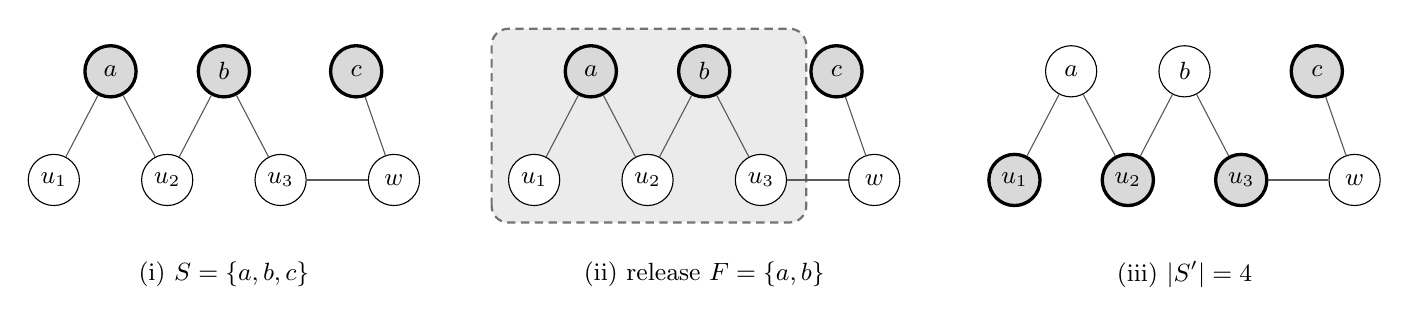
\begin{tikzpicture}[
  every node/.style={font=\small},
  vtx/.style={circle,draw,minimum size=6.5mm,inner sep=0pt,fill=white},
  ins/.style={vtx,fill=black!15,very thick},
  ed/.style={draw,black!65},
  x=12mm,y=12mm]

% ---- panel (i): the incumbent ----
\begin{scope}
  \node[ins] (a)  at (0,1.15)  {$a$};
  \node[ins] (b)  at (1.2,1.15){$b$};
  \node[ins] (c)  at (2.6,1.15){$c$};
  \node[vtx] (u1) at (-0.6,0) {$u_1$};
  \node[vtx] (u2) at (0.6,0)  {$u_2$};
  \node[vtx] (u3) at (1.8,0)  {$u_3$};
  \node[vtx] (w)  at (3.0,0)  {$w$};
  \foreach \s/\t in {a/u1,a/u2,b/u2,b/u3,c/w,u3/w} \draw[ed] (\s)--(\t);
  \node at (1.2,-1.0) {(i) $S=\{a,b,c\}$};
\end{scope}

% ---- panel (ii): the region ----
\begin{scope}[xshift=6.1cm]
  \node[ins] (a2)  at (0,1.15)  {$a$};
  \node[ins] (b2)  at (1.2,1.15){$b$};
  \node[ins] (c2)  at (2.6,1.15){$c$};
  \node[vtx] (u12) at (-0.6,0) {$u_1$};
  \node[vtx] (u22) at (0.6,0)  {$u_2$};
  \node[vtx] (u32) at (1.8,0)  {$u_3$};
  \node[vtx] (w2)  at (3.0,0)  {$w$};
  \begin{scope}[on background layer]
    \draw[rounded corners=6pt,fill=black!8,draw=black!55,thick,densely dashed]
      (-1.05,-0.45) rectangle (2.28,1.6);
  \end{scope}
  \foreach \s/\t in {a2/u12,a2/u22,b2/u22,b2/u32,c2/w2,u32/w2} \draw[ed] (\s)--(\t);
  \node at (1.2,-1.0) {(ii) release $F=\{a,b\}$};
\end{scope}

% ---- panel (iii): after the move ----
\begin{scope}[xshift=12.2cm]
  \node[vtx] (a3)  at (0,1.15)  {$a$};
  \node[vtx] (b3)  at (1.2,1.15){$b$};
  \node[ins] (c3)  at (2.6,1.15){$c$};
  \node[ins] (u13) at (-0.6,0) {$u_1$};
  \node[ins] (u23) at (0.6,0)  {$u_2$};
  \node[ins] (u33) at (1.8,0)  {$u_3$};
  \node[vtx] (w3)  at (3.0,0)  {$w$};
  \foreach \s/\t in {a3/u13,a3/u23,b3/u23,b3/u33,c3/w3,u33/w3} \draw[ed] (\s)--(\t);
  \node at (1.2,-1.0) {(iii) $|S'|=4$};
\end{scope}
\end{tikzpicture}
}
\caption{A region move that no $(1,k)$-swap expresses. Shaded
vertices are in the current solution. In (i) the incumbent $S=\{a,b,c\}$ is
maximal, so no vertex can simply be added. Releasing any \emph{single} vertex
also achieves nothing: $R(\{a\})=\{a,u_1\}$, $R(\{b\})=\{b,u_3\}$ and
$R(\{c\})=\{c,w\}$ each admit an independent set of size one, so every
$(1,k)$-swap returns the incumbent. Releasing $a$ and $b$ together gives the
region in (ii), $R(\{a,b\})=\{a,b,u_1,u_2,u_3\}$, because $u_2$ is the vertex
whose two incumbent neighbours are exactly $a$ and $b$. That region contains the
independent set $\{u_1,u_2,u_3\}$ of size three against the two vertices
released, and (iii) is the result: $|S'|=4$, which is $\alpha(G)$ here. Note that
$w$ stays outside the region --- its incumbent neighbour $c$ is not released ---
and that the edge $u_3w$ leaves the region. Theorem~\ref{thm:region}(a) forbids
edges from $R(F)$ to $S \setminus R(F)$ only, which is what makes the
substitution safe; edges to the rest of $V$ are unconstrained.}
\label{fig:region}
\end{figure}

Figure~\ref{fig:region} is a schematic with seven vertices. Figure~\ref{fig:move}
shows the same move on a real mesh, produced by the construction and the exact
solve described in this paper on a 90-point Delaunay graph; it is a worked example
that was found by searching for a move with positive gain, not a typical move,
and most moves find nothing.

\begin{figure}[htbp]
\centering
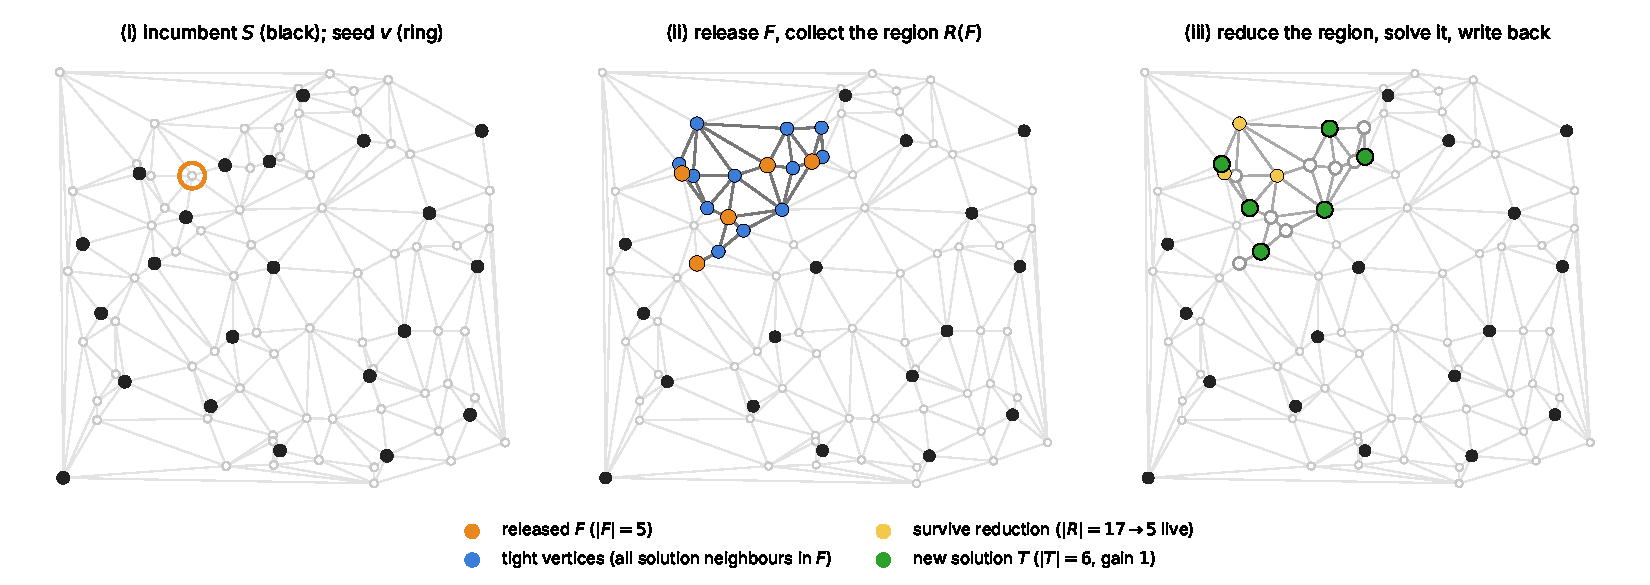
\includegraphics[width=\textwidth]{figures/move_example}
\caption{One region move on a Delaunay graph with 90 vertices. (i)~A maximal
independent set $S$ (black) and the seed vertex $v$ of the walk. (ii)~The walk
collects the first $k=5$ incumbent vertices it meets (orange, the released set
$F$); the blue vertices are those whose solution neighbours all lie in $F$. The
orange and blue vertices together are the region $R(F)$, and the heavy edges are
the edges of $G[R(F)]$. Every other vertex keeps a neighbour in $S\setminus F$,
so nothing outside can be affected. (iii)~The root reduction pass (degree-one and
domination rules here) settles 12 of the 17 region vertices, leaving 5 to branch
on (yellow); the exact solution (green) has 6 vertices against the 5 released, so
the incumbent grows by one. Each panel shows the whole graph, so the small size of
the region against the graph is visible.}
\label{fig:move}
\end{figure}

\paragraph{Cost of a move} With $t(u)=|N(u)\cap S|$ maintained incrementally,
$R(F)$ is built from a given $F$ in $O(\sum_{v\in F}\deg v)$: count for each outside
neighbour of $F$ how many of its neighbours lie in $F$, and admit it when the count
equals $t(u)$. Selecting $F$ is a separate cost: the implementation grows $F$ by a
breadth-first walk from a seed, collecting incumbent vertices until the target size
is reached and capping the vertices visited. The walk scans the full adjacency of
each vertex it visits, so a move is bounded by the total degree of the visited ball
and of the region, not by $|F|$; the largest degree in our benchmark is $100{,}029$.
The exact sub-solve is performed on the kernel of $G[R(F)]$ rather than on
$G[R(F)]$ itself.

\paragraph{Relation to classical swaps} For $F=\{v\}$, $R(F)$ is the set examined by
a $(1,2)$-swap \citep{andrade2012}, and solving $G[R(F)]$ finds the best $(1,k)$-swap
at $v$ for every $k$ at once. More generally, a move that releases $j$ vertices and
writes back $k$ \emph{is} a $(j,k)$-swap, so the neighbourhood is not a new class of
move. What Theorem~\ref{thm:region} supplies is a way to search it: the best
$(j,k)$-swap at $F$ over all $k$ is one induced subproblem, with no consistency check
against the rest of the incumbent, which is what makes $j$ in the tens affordable
where implementations that enumerate swaps are confined to $j\le 2$.

\section{Algorithm and implementation}
\label{sec:algorithm}

\subsection{The search}\label{sec:search}

Algorithm~\ref{alg:cascade} gives the overall structure. Kernelization runs
once; a \emph{dive} then constructs an initial solution by repeatedly discarding
a maximum-degree vertex and re-reducing, which reproduces reducing-peeling
\citep{chang2017}; the remaining budget goes to region moves. The step that
distinguishes the method is that the reduction rules are applied \emph{inside}
each move, to the region rather than to the input, which is what makes solving the
region exactly affordable.

\begin{algorithm}
\caption{\textsc{Cascade}: static region-move search}
\label{alg:cascade}
\small
\begin{algorithmic}[1]
\Require graph $G=(V,E)$, wall-clock budget $B$, seed; parameters of Table~\ref{tab:params}
\Ensure a maximal independent set $S^\star$ of $G$ (best found within $B$)
\State $(K,\mathit{trail}) \gets \textsc{Reduce}(G)$ \Comment{full rules; stops after $\kappa B$}
\State dive on $K$: discard a maximum-degree vertex, re-reduce (cheap rules), until $K=\emptyset$
\State $S \gets \textsc{Maximalise}(\textsc{Lift}(\mathit{trail}))$;\; $S^\star \gets S$
\State $W \gets$ shuffled kernel vertices and their neighbours;\; $k \gets k_0$;\; $\mathit{plateau}\gets\textbf{false}$
\While{time remains}
  \Repeat \Comment{one batch of $64$ region moves}
    \If{$W$ is empty} \Comment{a sweep has finished}
      \If{the sweep gained nothing} $\mathit{plateau}\gets\textbf{true}$;\; $k \gets k + \lfloor k/4\rfloor + 1$ \textbf{else} $\mathit{plateau}\gets\textbf{false}$
      \EndIf
      \State refill $W$ with all seeds, shuffled
    \EndIf
    \State $v \gets W.\textsc{pop}()$
    \State $F \gets$ first $k$ incumbent vertices on a BFS walk from $v$ \Comment{$\le\max(64,64k)$ visited}
    \State $R \gets F \cup \{u \notin S : N(u) \cap S \subseteq F\}$;\; build $G[R]$
    \State $T \gets \textsc{BranchAndReduce}(G[R])$ within node budget $\nu$, time slice $\sigma$
    \If{$|T| > |F|$ \textbf{or} ($|T|=|F|$, $T\neq F$ \textbf{and} $\mathit{plateau}$)}
      \State $S \gets (S \setminus R) \cup T$;\; add any vertex left with no neighbour in $S$; push $R\cup N(R)$ onto $W$
    \EndIf
    \If{$T$ not proved optimal \textbf{or} $|R|>\rho$} $k \gets \max(1,\lfloor k/2\rfloor)$;\; re-queue $v$
    \ElsIf{no gain} \textbf{if} $s$ consecutive proved moves without gain \textbf{then} $k \gets \min(k_{\max},2k)$
    \EndIf
  \Until{64 moves done}
  \State $S^\star \gets \max(S^\star, S)$
  \State \textsc{Perturb}$(S)$: force $q$ random kernel-side vertices in, evict their neighbours, run $24$ region moves; keep if not worse, else undo
  \If{$q$ at its maximum and $r$ consecutive kicks failed \textbf{or} no improvement for $\tau\times$(first-dive time)}
    \State \textbf{restart}: $S \gets$ fresh randomised dive; keep $S^\star$
  \EndIf
\EndWhile
\State \Return $S^\star$
\end{algorithmic}
\end{algorithm}

\begin{table}[htbp]
\centering
\caption{Parameters of Algorithm~\ref{alg:cascade} and their values in every
experiment (no per-family tuning). All are named by their flag in the
implementation.}
\label{tab:params}
\small
\begin{tabular}{llp{7.2cm}}
\toprule
Symbol & Value & Meaning \\
\midrule
$\kappa$ & 0.3 & share of $B$ that kernelization may use (\texttt{kernel\_share}) \\
$k_0$, $k_{\max}$ & 4, 4096 & initial and maximum number of released vertices (\texttt{lns\_start\_free}, \texttt{lns\_max\_free}) \\
$s$ & 512 & fruitless proved moves before $k$ doubles (\texttt{lns\_stale\_grow}) \\
$\rho$ & 3000 & region size above which the region is treated as too large (\texttt{lns\_region\_cap}) \\
$\nu$, $\sigma$ & 20\,000 nodes, 0.05\,s & sub-solve budgets; both grow (to $10^6$ nodes, 1\,s) after each fruitless sweep \\
$q$ & $1\to 32$ & kick strength; doubles after 32 consecutive failed kicks (\texttt{perturb\_max\_strength}) \\
$r$ & 200 & failed full-strength kicks before a restart (\texttt{restart\_after}) \\
$\tau$ & 200 & restart after this many first-dive durations without improvement (\texttt{restart\_idle\_dives}) \\
\bottomrule
\end{tabular}
\end{table}

The inner loop therefore has two clocks. \emph{Within} a sweep, $k$ halves when
a region is too large or its sub-solve is cut off, and doubles when $s=512$
consecutive regions were solved to proven optimality without a gain. \emph{Between}
sweeps, a sweep with no gain at all raises $k$ by a quarter, switches on
plateau moves, and enlarges the sub-solve budgets. Plateau moves accept a region
optimum that equals the released set in size but differs from it; randomised
tie-breaking in the sub-solver makes repeated solves of one region return
different optima. A perturbation runs after every batch of 64 region moves.

\paragraph{Reading Algorithm~\ref{alg:cascade}} Lines 1--3 build the starting
solution: reduce the graph, dive until nothing is left (each step discards one
maximum-degree vertex and re-reduces), then lift the result back to $G$. This part is
reducing-peeling \citep{chang2017} and everything after it only improves on it.
Lines 4--5 set up the worklist $W$ of seed vertices (the kernel and its neighbours,
since a settled vertex cannot be part of an improvement) and the first value of $k$.
Lines 6--22 are one batch of 64 region moves, drawn in
Figure~\ref{fig:flow}: take a seed, walk to find the $k$ released vertices
(line 13), build the region and solve it (lines 14--15), accept the result if it is
larger, or equal and on a plateau (lines 16--18), and adjust $k$ (lines 19--21). Line
23 keeps the best solution seen. Lines 24--27 are the escape mechanisms and run
once per batch, not once per move.

\begin{figure}[htbp]
\centering
\resizebox{\textwidth}{!}{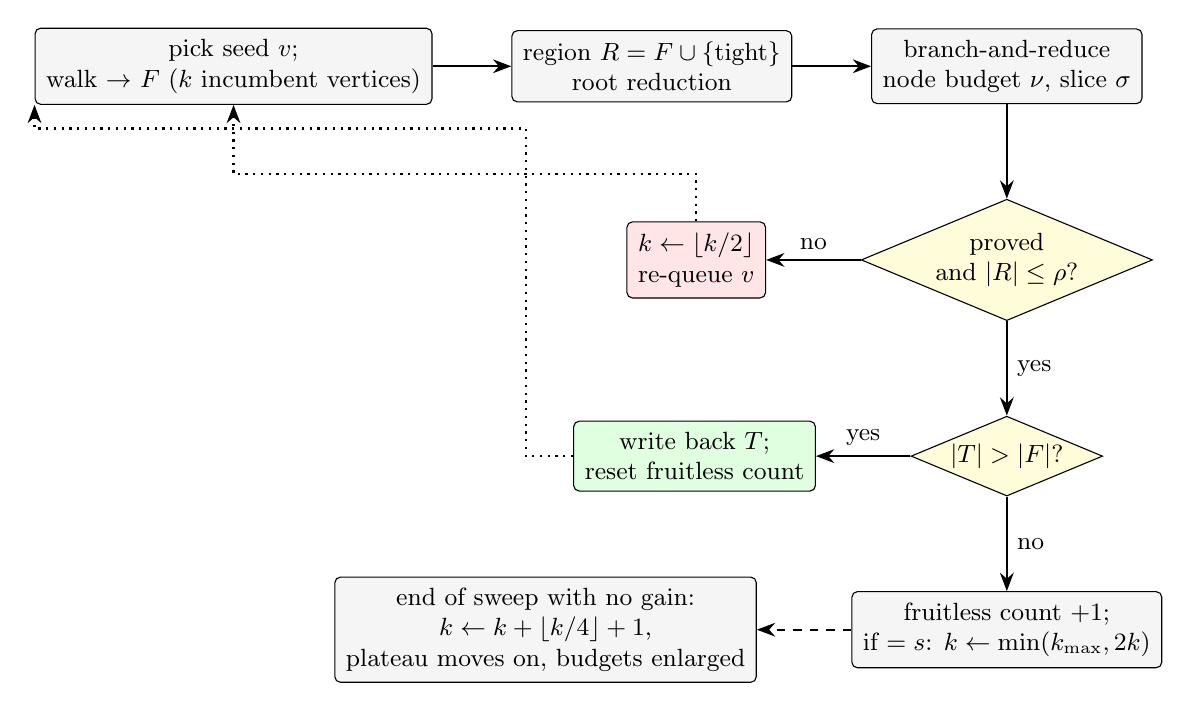
\begin{tikzpicture}[
  every node/.style={font=\small},
  box/.style={draw,rounded corners=2pt,align=center,minimum height=8mm,inner sep=4pt,fill=black!4},
  dec/.style={draw,diamond,aspect=2.4,align=center,inner sep=1pt,fill=yellow!15},
  act/.style={draw,rounded corners=2pt,align=center,inner sep=4pt,fill=green!12},
  bad/.style={draw,rounded corners=2pt,align=center,inner sep=4pt,fill=red!10},
  arr/.style={-{Stealth},thick},
  node distance=9mm]
\node[box] (walk) {pick seed $v$;\\ walk $\to$ $F$ ($k$ incumbent vertices)};
\node[box,right=10mm of walk] (reg) {region $R=F\cup\{\text{tight}\}$\\ root reduction};
\node[box,right=10mm of reg] (solve) {branch-and-reduce\\ node budget $\nu$, slice $\sigma$};
\node[dec,below=12mm of solve] (ok) {proved\\ and $|R|\le\rho$?};
\node[bad,left=12mm of ok] (halve) {$k\leftarrow\lfloor k/2\rfloor$\\ re-queue $v$};
\node[dec,below=12mm of ok] (gain) {$|T|>|F|$?};
\node[act,left=12mm of gain] (accept) {write back $T$;\\ reset fruitless count};
\node[box,below=12mm of gain] (stale) {fruitless count $+1$;\\ if $=s$: $k\leftarrow\min(k_{\max},2k)$};
\node[box,left=12mm of stale] (sweep) {end of sweep with no gain:\\ $k\leftarrow k+\lfloor k/4\rfloor+1$,\\ plateau moves on, budgets enlarged};
\draw[arr] (walk)--(reg); \draw[arr] (reg)--(solve); \draw[arr] (solve)--(ok);
\draw[arr] (ok)--node[above]{no} (halve); \draw[arr] (ok)--node[right]{yes} (gain);
\draw[arr] (gain)--node[above]{yes} (accept); \draw[arr] (gain)--node[right]{no} (stale);
\draw[arr,dashed] (stale)--(sweep);
\draw[arr,dotted] (halve.north) -- ++(0,0.6) -| (walk.south);
\draw[arr,dotted] (accept.west) -- ++(-0.6,0) |- ([yshift=-3mm]walk.south west) -- (walk.south west);
\end{tikzpicture}
}
\caption{One iteration of the inner loop (lines 12--21 of
Algorithm~\ref{alg:cascade}). Solid arrows are the main flow, dotted arrows return
to the next seed, and the dashed arrow is the sweep-level update. The two
adjustments of $k$ run in opposite directions: a failed sub-solve halves it, and a
long run of proved regions without a gain doubles it.}
\label{fig:flow}
\end{figure}

\begin{figure}[htbp]
\centering
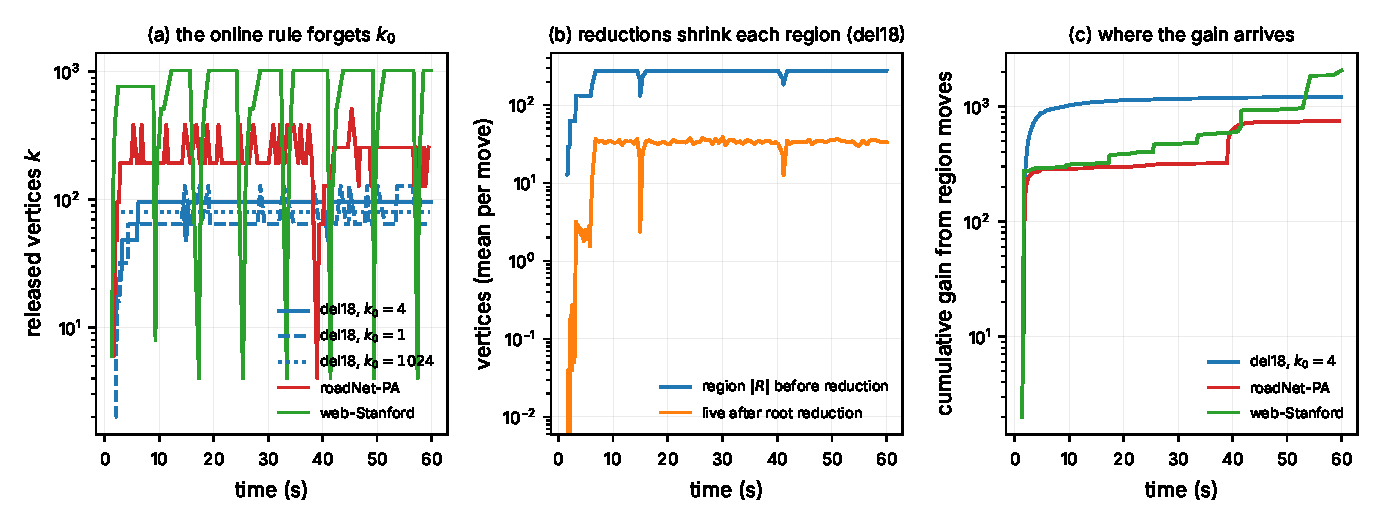
\includegraphics[width=\textwidth]{figures/adapt}
\caption{The size-control rule in operation (60\,s runs, one window per 500 region
moves). (a)~The number of released vertices $k$ against time. On \texttt{del18} it
settles near 80--100 whether the start is $k_0=1$, $4$ or $1024$; the sharp drops
on \texttt{web-Stanford} and \texttt{roadNet-PA} are restarts, which reset $k$ to
$k_0$. (b)~On \texttt{del18} the mean region has a few hundred vertices before the
root reduction pass and tens after it; this gap is what the reductions buy.
(c)~Cumulative gain from region moves: most of it arrives in the first
seconds on \texttt{del18} and \texttt{roadNet-PA}, in line with the small effect of a longer budget (Online Resource 1).}
\label{fig:adapt}
\end{figure}

\paragraph{The decision-space move} An alternative move rewinds the stack of dive
decisions to a chosen level, reverses the decision there and re-dives. It was our
first design and is the \textsc{dive} variant of the ablation
(Section~\ref{sec:ablation}); it has no separation property and is not a default.

\paragraph{Where the search looks} Every vertex decided by a reduction belongs
to some maximum independent set, so an improving move must touch a vertex that
survived into the kernel. Seeding the sweep from the kernel and its neighbours
rather than from all of $V$ matters on graphs that reduce well: a graph such as
\texttt{com-lj} has four million vertices and reduces to $1781$ at a fixed point
(Table~\ref{tab:kernels}).

\paragraph{Escaping local optima} Because region moves never degrade the incumbent,
the search stalls at a solution that is optimal for every region of the current
size. \emph{Plateau moves} (above) and \emph{perturbation}, which forces a vertex into
the solution, evicts its blocking neighbours, lets region moves repair the damage and
rolls back through a change log if the result is worse, address this. \emph{Restarts}
discard the incumbent and dive again, keeping the best solution in an archive; the
trigger is idle time in multiples of the cost of one dive, since a restart must pay for
a re-dive, so the smallest instances restart hundreds of times in a minute and the
largest never.

\subsection{Data structures and throughput}
\label{sec:implementation}

Reductions and branching decisions mutate the graph and must be reversible at every
node of a sub-search and after every region move. We use a compressed adjacency
array in which each entry stores the position of its twin, with a per-vertex pointer
separating live from dead neighbours; deleting a vertex swaps its entry to the end of
each live neighbour's range and decrements the pointer, and undoing it increments the
pointers again, both in $O(\deg v)$ with no payload. Degree-2 folding adds edges that
go into append-only per-vertex overflow lists, undone by a pop. Each node of a
sub-search owns an exact list of its live vertices; an earlier version that shared one
list could drop a vertex created by a fold, so the clique-cover bound came out too
small and pruned optimal solutions while still reporting a proof. The sub-solver is
reused across moves, since at a hundred thousand moves per minute its set-up would
cost more than the search. Kernelization gets a fixed share $\kappa=0.3$ of the
budget and is stopped where it stands when that is spent: on \texttt{soc-pokec},
running the rules to a fixed point takes $180$--$332$\,s, several times the whole
60-second budget, so a solver that insisted on finishing would return nothing. In the
ablation runs (three seeds, three processes sharing the machine) the full
configuration kernelizes \texttt{del18} in $1.6$--$2.0$\,s, completes the first dive in
a further $0.55$--$0.63$\,s and performs $102\,906$--$112\,414$ region moves in the
rest of 60\,s, one every $560\,\mu$s. Correctness is checked against exhaustive search
on random graphs with each rule disabled in turn, and every solution our solver reports
is verified independent and maximal. Further implementation notes are in the
supplement.
\section{Computational study}
\label{sec:experiments}

\subsection{Setup and instances}
\label{sec:setup-machine}

Runs are single-threaded on a four-core Intel Xeon at 2.10\,GHz with 15\,GB of
memory under Ubuntu 24.04, every solver compiled by GCC 13.3 at \texttt{-O3} and
given the same wall-clock budget, measured around the whole process so that reading
the instance and any construction phase are charged to the solver. Baselines are
built from their authors' sources: ReduMIS and OnlineMIS from KaMIS
\citep{lamm2017,dahlum2016}, reducing-peeling and near-linear kernelization (NearLinear,
LinearTime) from the release of \citet{chang2017}, and NuMVC and FastVC from a library
carrying the original implementations; the last two solve vertex cover and their
output is converted to an independent set. Each solver reads the format its own
implementation expects, converted by one tool distributed with our code.

Generative AI tools were used to assist with drafting and language editing of the manuscript text and with the preparation of scripts; the author reviewed the content, ran and checked every experiment, and is responsible for the work. Every value is checked independently where the solver emits its set: a separate
program re-reads the instance and confirms that the set contains no edge. The
exception is NearLinear and LinearTime, which print a size without the set; their
values are included, marked unverified in the raw records, and taken on trust (all 54
of their runs), as is one run each of ReduMIS and NuMVC (the instance on which they
returned nothing).

The benchmark has 27 instances in five families: Delaunay triangulations and random
geometric graphs (generated, fixed seed), road networks, social and web graphs (SNAP)
and the BHOSLIB \texttt{frb} collection \citep{xu2007}. The BHOSLIB instances are
distributed in \emph{clique} form, and the copies in common repositories are the
dense clique graphs (\texttt{frb30-15-1} there has 83,198 edges and independence
number 15); the instance for this problem is the complement, with 17,827 edges and
independence number 30, and that is what we use. Provenance, checksums and
preprocessing rules are in Online Resource 1; isolated vertices are kept, since removing
$q$ of them lowers the independence number by exactly $q$.

\begin{table}[htbp]
\centering
\caption{Size of the independent set found within the 60\,s budget (larger is better), all 27 instances. Best value per instance in bold; -- means no solution within the cutoff. Family order: geometric, road, social, web, BHOSLIB.}
\label{tab:quality}
\footnotesize
\fittable{\begin{tabular}{llrrrrrrrr}
\toprule
Instance & Family & $n$ & \textsc{Cascade} & ReduMIS & OnlineMIS & NearLinear & LinearTime & NuMVC & FastVC \\
\midrule
\texttt{rgg16} & geometric & 65501 & \textbf{16086} & \textbf{16086} & 16082 & 16035 & 15321 & 15905 & 16085 \\
\texttt{del16} & geometric & 65536 & \textbf{20647} & 20640 & 20630 & 20284 & 20213 & 20180 & 20638 \\
\texttt{rgg18} & geometric & 262011 & \textbf{64278} & \textbf{64278} & 63912 & 64094 & 61282 & 62548 & 64242 \\
\texttt{del18} & geometric & 262144 & \textbf{82656} & 82385 & 82019 & 81211 & 80881 & 80695 & 82579 \\
\texttt{rgg20} & geometric & 1048171 & \textbf{256994} & \textbf{256994} & 242366 & 256277 & 244769 & 239118 & 256680 \\
\texttt{del20} & geometric & 1048576 & \textbf{330066} & 321566 & 311146 & 324619 & 323438 & 311421 & 329802 \\
\midrule
\texttt{roadNet-PA} & road & 1088092 & 533627 & \textbf{533628} & 515876 & 531184 & 530910 & 513067 & 532571 \\
\texttt{roadNet-CA} & road & 1965206 & \textbf{961851} & \textbf{961851} & 924236 & 957199 & 956573 & 915797 & 959909 \\
\midrule
\texttt{ca-AstroPh} & social & 18772 & \textbf{6760} & \textbf{6760} & \textbf{6760} & \textbf{6760} & 6759 & \textbf{6760} & \textbf{6760} \\
\texttt{ca-CondMat} & social & 23133 & \textbf{9612} & \textbf{9612} & 9601 & \textbf{9612} & 9611 & 9611 & \textbf{9612} \\
\texttt{email-Enron} & social & 36692 & \textbf{22255} & \textbf{22255} & 22227 & \textbf{22255} & \textbf{22255} & 22253 & \textbf{22255} \\
\texttt{com-dblp} & social & 317080 & \textbf{152131} & \textbf{152131} & 152061 & \textbf{152131} & 152129 & 152112 & \textbf{152131} \\
\texttt{com-amazon} & social & 334863 & \textbf{174632} & \textbf{174632} & 172685 & 174627 & 174612 & 174510 & 174605 \\
\texttt{com-youtube} & social & 1134890 & \textbf{857945} & \textbf{857945} & 857680 & \textbf{857945} & 857944 & 857708 & \textbf{857945} \\
\texttt{soc-pokec-relationships} & social & 1632803 & 788866 & -- & 776663 & 789161 & 789003 & 787320 & \textbf{789352} \\
\texttt{as-skitter} & social & 1696415 & 1170576 & \textbf{1170580} & 1152300 & 1170541 & 1170410 & 1168352 & 1168417 \\
\texttt{wiki-Talk} & social & 2394385 & \textbf{2338222} & \textbf{2338222} & 2338207 & \textbf{2338222} & \textbf{2338222} & 2338220 & \textbf{2338222} \\
\texttt{com-lj} & social & 3997962 & \textbf{2085626} & \textbf{2085626} & 2066610 & 2085604 & 2085353 & -- & 2085169 \\
\midrule
\texttt{web-Stanford} & web & 281903 & 163375 & \textbf{163390} & 162453 & 163198 & 163121 & 162453 & 162953 \\
\texttt{web-BerkStan} & web & 685230 & 408380 & \textbf{408482} & 406062 & 408054 & 407716 & 405003 & 406323 \\
\midrule
\texttt{frb30-15-1} & bhoslib & 450 & \textbf{30} & \textbf{30} & 29 & 24 & 22 & \textbf{30} & \textbf{30} \\
\texttt{frb35-17-1} & bhoslib & 595 & 34 & \textbf{35} & 33 & 27 & 25 & \textbf{35} & \textbf{35} \\
\texttt{frb40-19-1} & bhoslib & 760 & 39 & \textbf{40} & 39 & 27 & 29 & \textbf{40} & \textbf{40} \\
\texttt{frb45-21-1} & bhoslib & 945 & 43 & 43 & 42 & 33 & 32 & \textbf{45} & \textbf{45} \\
\texttt{frb50-23-1} & bhoslib & 1150 & 48 & 49 & 48 & 35 & 33 & \textbf{50} & 49 \\
\texttt{frb53-24-1} & bhoslib & 1272 & 50 & 51 & 49 & 38 & 40 & \textbf{52} & 51 \\
\texttt{frb59-26-1} & bhoslib & 1534 & 56 & 57 & 56 & 43 & 43 & \textbf{58} & 56 \\
\bottomrule
\end{tabular}}
\end{table}

\begin{table}[htbp]
\centering
\caption{Aggregate over all 27 instances. The gap of an algorithm on an instance is $(\text{best of the seven algorithms} - \text{its value}) / \text{best of the seven algorithms listed}$.}
\label{tab:aggregate}
\begin{tabular}{lrrrr}
\toprule
Algorithm & \#best & \#solved & mean gap & max gap \\
\midrule
\textsc{Cascade} & 16 & 27 & 0.785\% & 4.444\% \\
ReduMIS & 19 & 26 & 0.501\% & 4.444\% \\
OnlineMIS & 1 & 27 & 2.156\% & 6.667\% \\
NearLinear & 6 & 27 & 7.113\% & 32.500\% \\
LinearTime & 2 & 27 & 8.019\% & 34.000\% \\
NuMVC & 8 & 26 & 1.219\% & 6.956\% \\
FastVC & 11 & 27 & 0.340\% & 3.448\% \\
\bottomrule
\end{tabular}
\end{table}

\begin{table}[htbp]
\centering
\caption{Paired Wilcoxon signed-rank test of \textsc{Cascade} against each baseline over the instances both solved, at the 60\,s budget, computed on relative gaps to the best of the seven solvers. $p_{\mathrm{Holm}}$ is Holm-adjusted over the six comparisons; a verdict names the better solver when $p_{\mathrm{Holm}}<0.05$.}
\label{tab:wilcoxon}
\fittable{
\begin{tabular}{lrrrrrrr}
\toprule
Baseline & pairs & win & tie & loss & $p$ & $p_{\mathrm{Holm}}$ & verdict \\
\midrule
ReduMIS & 26 & 3 & 14 & 9 & 0.1268 & 0.3805 & -- \\
OnlineMIS & 27 & 23 & 4 & 0 & $<10^{-4}$ & $<10^{-4}$ & \textsc{Cascade} \\
NearLinear & 27 & 20 & 6 & 1 & $<10^{-4}$ & 0.0002 & \textsc{Cascade} \\
LinearTime & 27 & 24 & 2 & 1 & $<10^{-4}$ & 0.0001 & \textsc{Cascade} \\
NuMVC & 26 & 18 & 2 & 6 & 0.1549 & 0.3805 & -- \\
FastVC & 27 & 13 & 8 & 6 & 0.4406 & 0.4406 & -- \\
\bottomrule
\end{tabular}
}
\end{table}


\subsection{Solution quality and aggregate comparison}

Table~\ref{tab:quality} gives the size each solver returned; per-family tables, the
decomposition of the comparison with ReduMIS and the budget actually used by each
solver are in Online Resource 1. \textsc{Cascade} attains the best value of the seven
solvers on every geometric instance and is strictly ahead on the three Delaunay
graphs, by $+7$, $+77$ and $+264$ vertices over the strongest baseline on each
($0.03\%$, $0.09\%$ and $0.08\%$; ReduMIS on \texttt{del16}, FastVC on the others). Against
ReduMIS alone the margins are $+7$, $+271$ and $+8500$, but the last is largely a
statement about convergence rate: at ten times the budget it shrinks to $+1550$ while
the margin over the strongest baseline is unchanged (Online Resource 1). On the random
geometric graphs \textsc{Cascade} and ReduMIS reach the same value, which the exact
solvers prove optimal for \texttt{rgg16} and \texttt{rgg18}. On road networks and most
social graphs the strong solvers agree to within a handful of vertices because the
kernels are small, and what separates them is robustness: ReduMIS returned nothing on
\texttt{soc-pokec} within eleven minutes and NuMVC nothing on \texttt{com-lj} within
sixteen, while \textsc{Cascade} returned a verified solution on every instance. On web
graphs it is behind ReduMIS by 15 and 102 vertices ($0.009\%$ and $0.025\%$) and on
\texttt{soc-pokec} $0.06\%$ behind FastVC. On BHOSLIB it is the weaker tool: it reaches
the optimum of \texttt{frb30-15-1} but is one or two vertices short of the best value
on the other six, always NuMVC's or FastVC's (45 against our 43 on
\texttt{frb45-21-1}, a $4.4\%$ gap, the largest we record). On a dense graph almost
every outside vertex has several incumbent neighbours, so releasing a small $F$
unlocks nothing and a large one makes the region the whole graph; the move degenerates
and specialised local search is the better tool.

\paragraph{Reference sets} Three reference sets appear and are not interchangeable.
(i)~\emph{Best of the other six}: against it \textsc{Cascade} is strictly ahead on 3
instances, ties on 13 and is behind on 11, i.e.\ it attains the best of all seven on
$3+13=16$; these are the counts in the abstract and in Table~\ref{tab:aggregate}.
(ii)~\emph{Best of the seven}: the denominator of the gaps in Table~\ref{tab:aggregate}
and of the Wilcoxon tests. (iii)~\emph{ReduMIS alone}: 26 instances, since ReduMIS
returned nothing on \texttt{soc-pokec}; \textsc{Cascade} is ahead on 3, level on 14
and behind on 9. An earlier version of this study built the quality tables from five of
the seven solvers; all tables here include all seven.

\paragraph{Aggregate} The mean relative gap of \textsc{Cascade} is $0.785\%$, against
$0.340\%$ for FastVC, $0.501\%$ for ReduMIS and $1.219\%$ for NuMVC, so by that
statistic it is third of seven, because its worst instances are the dense BHOSLIB ones.
The Wilcoxon tests (Table~\ref{tab:wilcoxon}) are run on relative gaps and
Holm-corrected over the six comparisons. They find \textsc{Cascade} significantly
better than OnlineMIS, NearLinear and LinearTime and \emph{no significant difference}
from ReduMIS ($p_{\mathrm{Holm}}=0.38$), NuMVC ($0.38$) or FastVC ($0.44$). Two of the
three significant comparisons are against the unverified reducing-peeling programs. The
reading is that the strong solvers are equal on most of this benchmark, that
\textsc{Cascade} degrades more gracefully on the largest geometric instance, and that
ReduMIS holds a small edge on web graphs.

\subsection{Residual kernels and direct exact solving}
\label{sec:kernels}

The motivation for region moves is a large residual kernel, so the first measurement
is how large the kernel is on this benchmark and whether it could simply be solved
exactly. Table~\ref{tab:kernels} reports, for the 19 instances that can be rebuilt
(BHOSLIB excluded), the kernel left under the 60\,s run's own rule (kernelization
limited to $\kappa=0.3$ of the budget), the kernel at a fixed point, and the result of
running the exact engine of Section~\ref{sec:implementation} on the whole input for
120\,s (\textsc{Cascade}\,\texttt{--exact}: the same reductions, then
branch-and-reduce). These runs were made on a different, shared machine from the main
tables, with three processes at a time, so times are only indicative.

\begin{table}[htbp]
\centering
\caption{Residual kernel after reduction, and the whole-input exact solve. \emph{Capped}: kernelization under the 60\,s run's own rule (a share $\kappa=0.3$ of the budget). \emph{Full}: run to a fixed point (limit 300\,s). \emph{Exact}: \textsc{Cascade}\,\texttt{--exact} on the whole input, limit 120\,s; time to a proven optimum, or the best value if not proved. Kernel size is the number of vertices left.}
\label{tab:kernels}
\small
\fittable{
\begin{tabular}{lrrrrrrrr}
\toprule
Instance & $n$ & capped $|K|$ & \% of $n$ & time (s) & full $|K|$ & time (s) & exact (s) & status \\
\midrule
\texttt{ca-AstroPh} & 18772 & 0 & 0.00 & 0.01 & 0 & 0.01 & 0.01 & proved \\
\texttt{ca-CondMat} & 23133 & 0 & 0.00 & 0.00 & 0 & 0.00 & 0.01 & proved \\
\texttt{email-Enron} & 36692 & 0 & 0.00 & 0.01 & 0 & 0.01 & 0.02 & proved \\
\texttt{rgg16} & 65501 & 686 & 1.05 & 0.20 & 686 & 0.28 & 120 & open \\
\texttt{del16} & 65536 & 55757 & 85.08 & 0.27 & 55757 & 0.21 & 120 & open \\
\texttt{rgg18} & 262011 & 3118 & 1.19 & 1.71 & 3118 & 1.26 & 120 & open \\
\texttt{del18} & 262144 & 221573 & 84.52 & 2.16 & 221573 & 3.32 & 148 & open \\
\texttt{web-Stanford} & 281903 & 9510 & 3.37 & 1.20 & 9510 & 1.52 & 120 & open \\
\texttt{com-dblp} & 317080 & 0 & 0.00 & 0.14 & 0 & 0.18 & 0.21 & proved \\
\texttt{com-amazon} & 334863 & 126 & 0.04 & 0.40 & 126 & 0.35 & 0.54 & proved \\
\texttt{web-BerkStan} & 685230 & 21743 & 3.17 & 2.03 & 21743 & 2.13 & 120 & open \\
\texttt{del20} & 1048576 & 893358 & 85.20 & 11.47 & 893358 & 17.56 & 278 & open \\
\texttt{roadNet-PA} & 1088092 & 44072 & 4.05 & 1.18 & 44072 & 0.93 & 120 & open \\
\texttt{com-youtube} & 1134890 & 0 & 0.00 & 0.63 & 0 & 0.59 & 0.86 & proved \\
\texttt{soc-pokec-relationships} & 1632803 & 1197405$^{\ast}$ & 73.33 & 18.02 & 686846 & 331.70 & 743 & no output \\
\texttt{as-skitter} & 1696415 & 4938 & 0.29 & 8.15 & 4938 & 8.71 & 120 & open \\
\texttt{roadNet-CA} & 1965206 & 67274 & 3.42 & 1.71 & 67274 & 2.04 & 120 & open \\
\texttt{wiki-Talk} & 2394385 & 0 & 0.00 & 1.41 & 0 & 1.87 & 1.28 & proved \\
\texttt{com-lj} & 3997962 & 212739$^{\ast}$ & 5.32 & 18.01 & 1781 & 24.30 & 120 & open \\
\bottomrule
\end{tabular}}
\\[2pt]\footnotesize $^{\ast}$ kernelization stopped by the budget share before a fixed point.
\end{table}


\emph{Kernel size is bimodal.} Six instances reduce to an empty kernel and a seventh to
126 vertices; there kernelization alone is optimal, direct exact solving proves it in
under 1.3\,s, and region moves have nothing to do. Road networks, random geometric
graphs, web graphs and \texttt{as-skitter} keep $0.3$--$4\%$ of their vertices (686 to
67\,274) and the Delaunay graphs $85\%$. None of the 12 instances with a non-trivial
kernel is solved by the exact engine in 120\,s (\texttt{del18} and \texttt{del20}
overran the limit because the reduction pass is not interruptible, and \texttt{soc-pokec}
produced no output in 743\,s for the same reason). So the premise of a hard residual
kernel holds on 12 of the 19 instances and not on the other seven.

\emph{Kernel size does not predict the margin.} Across the 19 instances the Spearman
correlation between retained fraction and relative margin over the best baseline is
$\rho=0.14$ ($p=0.56$); omitting the three Delaunay graphs it is $-0.57$ ($p=0.02$).
All three strict wins have a kernel of about $85\%$, but \texttt{soc-pokec}, with a
$73\%$ capped kernel, is a loss and the instances with $0.3$--$4\%$ kernels are ties or
small losses. A large kernel is therefore not sufficient. What the three wins share
beyond it is that they are planar, of bounded degree (at most 22) and generated by one
mechanism, and the benchmark contains no second family with that property.

\emph{Budget caps change what ``kernel'' means.} For \texttt{com-lj} and
\texttt{soc-pokec} the cap of $0.3B=18$\,s stops kernelization early on this machine,
and where it stops depends on speed: three runs of the same configuration left
\texttt{com-lj} with $3544$, $212\,739$ (reported) and $899\,607$ vertices (the last with
three processes sharing the machine), against $1781$ at a fixed point after 24\,s, and
\texttt{soc-pokec} with $73$--$75\%$ against $42\%$ after 332\,s. The residual a budgeted
run searches is a function of the budget and the machine as much as of the graph.

\subsection{Ablation}
\label{sec:ablation}

Table~\ref{tab:ablation} removes whole components: \textsc{no-lns} disables region
moves, leaving kernelization plus the greedy dive and restarts; \textsc{dive} replaces
the move with the decision-space move; \textsc{no-pert} removes perturbation and
restarts; \textsc{no-lp} removes the LP reduction. These are separate runs from the main
study, so the full column differs from Table~\ref{tab:quality} by a few vertices.
Removing region moves costs $1.2\%$ on \texttt{del18}, $1.4\%$ on \texttt{del16} (an order
of magnitude more than the margin over the strongest baseline) and $32.5\%$ on
\texttt{frb40-19-1}, $1577$ vertices summed over the seven instances; nothing else comes
close. The decision-space move recovers almost none of this on the large sparse
instances. Perturbation and the LP reduction are within noise, and on the family where
the margin lives the shipped configuration is not the best variant: without
perturbation and restarts \texttt{del16} returns 20\,656 against 20\,648, and without
the LP reduction \texttt{del18} returns 82\,666 against 82\,661. Both differences are of
the order of the seed spread ($0.024\%$), so they are not evidence that the components
hurt, nor that they help.

\begin{table}[htbp]
\centering
\caption{Ablation: each row disables one component. Values in brackets are the change from the full algorithm.}
\label{tab:ablation}
\small
\fittable{\begin{tabular}{lrrrrr}
\toprule
Instance & full & no region moves & no perturbation/restarts & no LP reduction & decision-space moves \\
\midrule
\texttt{del16} & 20648 & 20369 (-279) & 20656 (+8) & 20652 (+4) & 20383 (-265) \\
\texttt{del18} & 82661 & 81639 (-1022) & 82657 (-4) & 82666 (+5) & 81639 (-1022) \\
\texttt{rgg16} & 16086 & 16085 (-1) & 16086 (+0) & 16086 (+0) & 16086 (+0) \\
\texttt{roadNet-PA} & 533627 & 533385 (-242) & 533627 (+0) & 533627 (+0) & 533385 (-242) \\
\texttt{web-Stanford} & 163375 & 163369 (-6) & 163375 (+0) & 163373 (-2) & 163369 (-6) \\
\texttt{frb40-19-1} & 40 & 27 (-13) & 38 (-2) & 40 (+0) & 34 (-6) \\
\texttt{frb59-26-1} & 56 & 42 (-14) & 56 (+0) & 57 (+1) & 49 (-7) \\
\bottomrule
\end{tabular}}
\end{table}


\subsection{Exact against heuristic repair, and regional reductions}
\label{sec:regional}

Table~\ref{tab:ablation} does not separate the two ingredients of the method: that the
region is solved \emph{exactly} and that reductions run \emph{inside} it.
Table~\ref{tab:regional} does, under one implementation, one region-selection rule, one
budget and three seeds. \emph{Heuristic repair} applies the root reduction pass and then
one greedy pass (lowest degree first) with no branching and the same acceptance test
$|T|\ge|F|$; \emph{no regional reductions} runs the exact branch-and-bound on the raw
region. In both the online rule for $k$ is the same code, except that for heuristic
repair a sub-solve counts as ``solved'' whenever the region is below the size cap
$\rho$, since there is no proof signal.

\begin{table}[htbp]
\centering
\caption{Exact against heuristic repair, and regional reductions on and off, under one implementation, one region-selection rule and one 60\,s budget. Mean size over three seeds (bracket: change from the full configuration). The last three columns are process data for the full configuration on that instance (per region move, mean over seeds): vertices in the region before reduction, vertices left after the root reduction pass, and the share of sub-solves proved optimal.}
\label{tab:regional}
\small
\fittable{
\begin{tabular}{lrrrrrrr}
\toprule
Instance & exact repair, regional reductions (full) & heuristic repair (reduce, then one greedy pass) & exact repair, no regional reductions & no region moves & $|R|$ & $|R'|$ & proved \\
\midrule
\texttt{del16} & 20645.0 & 20614.3 (-30.7) & 20595.0 (-50.0) & 20376.3 (-268.7) & 89 & 4.8 & 100.0\% \\
\texttt{del18} & 82653.3 & 82510.0 (-143.3) & 82443.0 (-210.3) & 81635.0 (-1018.3) & 137 & 12.0 & 100.0\% \\
\texttt{rgg16} & 16086.0 & 16086.0 (+0.0) & 16086.0 (+0.0) & 16084.7 (-1.3) & 69 & 1.1 & 100.0\% \\
\texttt{roadNet-PA} & 533627.0 & 533607.0 (-20.0) & 533573.0 (-54.0) & 533375.3 (-251.7) & 203 & 16.5 & 100.0\% \\
\texttt{web-Stanford} & 163373.3 & 163369.7 (-3.7) & 163371.3 (-2.0) & 163365.0 (-8.3) & 396 & 21.5 & 100.0\% \\
\texttt{com-amazon} & 174632.0 & 174632.0 (+0.0) & 174632.0 (+0.0) & 174632.0 (+0.0) & 391 & 7.5 & 100.0\% \\
\bottomrule
\end{tabular}}
\end{table}


Exact repair with reductions is the best of the four on every instance and the others
are never ahead. On \texttt{del18}, heuristic repair loses 143 vertices and removing the
regional reductions 210, against 1018 for removing region moves altogether; on
\texttt{del16}, 31, 50 and 269; on \texttt{roadNet-PA}, 20, 54 and 252. The two
instances that reduce almost completely show no difference. The process columns show
why. Without reductions the sub-solver cannot afford large regions: $k$ settles at
$16$--$32$ and regions have $36$--$53$ vertices, against $k=64$--$256$ and regions of
$89$--$203$ vertices on the Delaunay and road instances in the full configuration, which
the root reduction pass collapses to $5$--$17$ live vertices (a factor of $11$--$19$).
With heuristic repair the rule has no brake and $k$ climbs to $512$--$1024$, so one
greedy pass is applied to regions of $177$--$589$ vertices. The proved share is near
$100\%$ in the full configuration by construction, since a failed sub-solve halves $k$;
the information is in the \emph{size} of the region it can hold. The move rate is
$1.3\times10^3$ to $8.4\times10^3$ per second.

\subsection{Independent Delaunay graphs}
\label{sec:delaunay}

All three strict wins are on one sample of one generator, so Table~\ref{tab:delaunay}
runs \textsc{Cascade} on six independent samples at $2^{16}$ and $2^{18}$ points
(generator seeds 1--6; seed 1 is the main-benchmark graph) and on the public DIMACS10
\texttt{delaunay\_n16}, \texttt{n18} and \texttt{n20}, three solver seeds each (two for
seeds 4--6).

\begin{table}[htbp]
\centering
\caption{\textsc{Cascade} on independent Delaunay graphs: seeds 1--6 of the generator and the public DIMACS10 \texttt{delaunay\_n} graphs, 60\,s. Solver seeds 1--3 (1--2 for $2^{16}$ and $2^{18}$ seeds 4--6; see text). Baselines were not run on these instances.}
\label{tab:delaunay}
\small
\fittable{\begin{tabular}{lrrrr}
\toprule
Instance & runs & min & mean & max \\
\midrule
\texttt{del16} & 3 & 20647 & 20648.0 & 20649 \\
\texttt{del18} & 3 & 82649 & 82651.3 & 82655 \\
\texttt{s2\slash del16} & 3 & 20693 & 20695.3 & 20697 \\
\texttt{s2\slash del18} & 3 & 82667 & 82670.3 & 82676 \\
\texttt{s3\slash del16} & 3 & 20655 & 20656.7 & 20658 \\
\texttt{s3\slash del18} & 3 & 82644 & 82651.3 & 82657 \\
\texttt{s4\slash del16} & 2 & 20689 & 20690.0 & 20691 \\
\texttt{s4\slash del18} & 2 & 82690 & 82691.0 & 82692 \\
\texttt{s5\slash del16} & 2 & 20639 & 20644.5 & 20650 \\
\texttt{s5\slash del18} & 2 & 82635 & 82638.0 & 82641 \\
\texttt{s6\slash del16} & 2 & 20672 & 20672.5 & 20673 \\
\texttt{s6\slash del18} & 2 & 82720 & 82722.5 & 82725 \\
DIMACS10 \texttt{delaunay\_n16} & 3 & 20688 & 20691.3 & 20694 \\
DIMACS10 \texttt{delaunay\_n18} & 3 & 82584 & 82585.7 & 82587 \\
DIMACS10 \texttt{delaunay\_n20} & 3 & 330164 & 330201.0 & 330229 \\
\bottomrule
\end{tabular}}
\end{table}


\emph{This experiment does not test the comparison}: the baselines were not run on these
graphs, so it says nothing about whether \textsc{Cascade} is ahead of ReduMIS or FastVC
on a new Delaunay graph. It does show how much a one-graph margin can mean. The mean over
solver seeds varies by $50.8$ vertices ($0.25\%$) across the six $2^{16}$ samples and by
$84.5$ ($0.10\%$) across the six $2^{18}$ samples, while the spread over solver seeds on
a fixed graph is at most 11 and 13, several times smaller than the between-sample range and
the margins claimed on the seed-1 graph ($0.03\%$, $0.09\%$). Such a margin is a paired
difference on one graph and cannot be extrapolated to the family without paired runs on
more samples.

\subsection{Parameter sensitivity}
\label{sec:sensitivity}

The online rule starts from $k_0=4$. Table~\ref{tab:ksweep} varies $k_0$ from $1$ to
$1024$ on four instances, one run per cell. On \texttt{del18} the results span
$82\,641$--$82\,660$ ($0.023\%$, the seed-to-seed spread of $0.024\%$), on
\texttt{web-Stanford} and \texttt{roadNet-PA} one or two vertices, and on \texttt{rgg16}
every setting returns 16\,086. The rule forgets its start where it matters: on
\texttt{del18} the final $k$ is $80$--$128$ for every $k_0$. Among the other parameters
(Online Resource 1) only \texttt{restart\_idle\_dives} is sensitive: it moves \texttt{del18}
by $0.081\%$, three times the seed spread, and restarting too eagerly costs quality
while restarting too lazily costs almost nothing.

\begin{table}[htbp]
\centering
\caption{Sensitivity to the initial number of released vertices $k_0$ (\texttt{--lns-free}); the online rule then adapts $k$. One run per cell, 60\,s. The last column is the final $k$ reached at $k_0=4$.}
\label{tab:ksweep}
\small
\fittable{\begin{tabular}{lrrrrrrr}
\toprule
Instance & $k_0=1$ & $k_0=4$ & $k_0=16$ & $k_0=64$ & $k_0=256$ & $k_0=1024$ & spread (\%) \\
\midrule
\texttt{del18} & 82651 & 82656 & 82660 & 82645 & 82641 & 82645 & 0.023 \\
\texttt{rgg16} & 16086 & 16086 & 16086 & 16086 & 16086 & 16086 & 0.000 \\
\texttt{web-Stanford} & 163374 & 163375 & 163374 & 163376 & 163374 & 163375 & 0.001 \\
\texttt{roadNet-PA} & 533626 & 533626 & 533627 & 533627 & 533627 & 533627 & 0.000 \\
\bottomrule
\end{tabular}}
\end{table}


\subsection{Seed study}

The solvers compared here are randomised, so we repeated a subset of ten
instances with five seeds each. Table~\ref{tab:seeds} reports the best and mean
size, and Figure~\ref{fig:seeds} the spread.

The single-seed picture holds, and no more than it. On best-of-five,
computed on relative gaps with Holm correction over four comparisons,
\textsc{Cascade} is significantly ahead of OnlineMIS ($p=0.0078$, adjusted
$0.047$) and indistinguishable from ReduMIS ($p=0.81$), NuMVC ($0.14$) and FastVC
($0.12$); on the mean over seeds the verdicts are the same (OnlineMIS $p=0.002$;
the others above $0.27$), with \textsc{Cascade} ahead of OnlineMIS on all ten
instances. NearLinear and LinearTime are deterministic and were not repeated.

The figure also shows a limitation. On every geometric, road and web instance
our solver's five runs collapse to a line: the spread is at most $0.024\%$, and
on two instances all five seeds return the same value. On the BHOSLIB instances
it widens by two orders of magnitude, to $2.5\%$ on \texttt{frb40-19-1} and
$2.0\%$ on \texttt{frb53-24-1}. It is not the most variable solver there ---
OnlineMIS spreads $5.1\%$ and $3.9\%$ on those two instances --- but it is
markedly less stable than ReduMIS and FastVC, which return the same value on
every seed of both, and on \texttt{frb40-19-1} that value is 40 against our 39
or 40. This is the same degeneracy discussed in
Section~\ref{sec:move} seen from another angle: when the region move cannot
find traction, what remains is the restart mechanism, and outcomes then depend
on which restart happens to land well. A practitioner running a single seed on a
dense instance should expect variance that the other families do not show.

\begin{table}[htbp]
\centering
\caption{Five seeds per instance at the 60\,s budget: best and mean size found. The spread is negligible on every family except BHOSLIB.}
\label{tab:seeds}
\small
\begin{tabular}{lrrrrr}
\toprule
Instance & \textsc{Cascade} & ReduMIS & FastVC & NuMVC & OnlineMIS \\
\midrule
\texttt{del16} & \textbf{20647 / 20644.2} & 20641 / 20639.4 & 20642 / 20637.0 & 20192 / 20178.2 & 20634 / 20631.6 \\
\texttt{del18} & \textbf{82656 / 82652.2} & 82393 / 82369.0 & 82589 / 82581.0 & 80727 / 80699.2 & 82042 / 82030.8 \\
\texttt{del20} & \textbf{330125 / 330104.2} & 321935 / 321503.0 & 329833 / 329818.2 & 311469 / 311427.0 & 311198 / 311117.6 \\
\texttt{frb40-19-1} & \textbf{40 / 39.6} & \textbf{40 / 40.0} & \textbf{40 / 40.0} & \textbf{40 / 39.8} & 39 / 38.4 \\
\texttt{frb53-24-1} & 51 / 50.4 & 51 / 51.0 & 51 / 51.0 & \textbf{52 / 52.0} & 51 / 50.0 \\
\texttt{frb59-26-1} & 56 / 56.0 & 57 / 57.0 & 57 / 56.6 & \textbf{58 / 58.0} & 56 / 55.8 \\
\texttt{rgg18} & \textbf{64278 / 64278.0} & \textbf{64278 / 64278.0} & 64255 / 64252.4 & 62550 / 62532.6 & 63911 / 63907.4 \\
\texttt{roadNet-PA} & \textbf{533628 / 533627.2} & \textbf{533628 / 533627.2} & 532575 / 532560.4 & 513102 / 513084.4 & 515949 / 515874.2 \\
\texttt{web-BerkStan} & 408402 / 408389.4 & \textbf{408482 / 408482.0} & 406338 / 406292.6 & 404996 / 404978.6 & 406051 / 405951.4 \\
\texttt{web-Stanford} & 163375 / 163373.0 & \textbf{163390 / 163390.0} & 162972 / 162964.8 & 162480 / 162461.6 & 162450 / 162433.8 \\
\bottomrule
\end{tabular}
\end{table}


\begin{figure}[htbp]
\centering
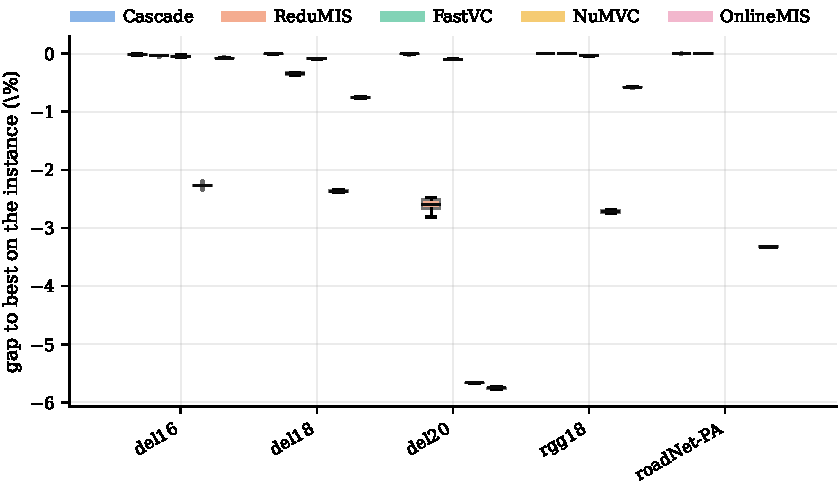
\includegraphics[width=\textwidth]{figures/seeds}
\caption{Spread over five seeds, as a percentage of the best value reached on
each instance. Boxes show the quartiles and the median; whiskers the range.}
\label{fig:seeds}
\end{figure}


\subsection{The long budget}
\label{sec:longbudget}

The main study gives every solver 60 seconds. That choice needs defending,
because a budget short enough to favour one convergence profile over another
would decide the comparison by itself. We therefore repeated four instances,
one per family, at ten times the budget. Table~\ref{tab:longbudget} gives the
result, and the comparison that matters is with the 60-second tables.

On three of the four instances the extra budget buys almost nothing.
\textsc{Cascade} and ReduMIS return \emph{exactly} the same value on
\texttt{roadNet-CA} and on \texttt{web-BerkStan} at 600 seconds as at 60, and on
\texttt{frb59-26-1} every solver moves by at most a single vertex. Those
instances are converged well inside the shorter budget, and nothing in the main
tables is an artefact of stopping early.

\texttt{del20} is the exception, and it qualifies our own headline. At 60
seconds \textsc{Cascade} leads ReduMIS there by 8500 vertices; at 600 seconds it
leads by 1550. ReduMIS gains 7417 vertices from the extra time and NuMVC 6227,
against 467 for \textsc{Cascade} and 390 for FastVC. The large gap to ReduMIS
that Section~\ref{sec:experiments} reports on the largest Delaunay instance is
therefore substantially a statement about convergence rate rather than about
final quality: ReduMIS gets to a similar place, it simply takes an order of
magnitude longer to do it.

Two things survive that correction. \textsc{Cascade} still returns the best value
on \texttt{del20} at the long budget, 330\,533 against FastVC's 330\,192, and its
margin over the \emph{strongest} baseline is essentially unchanged by the extra
time --- 264 vertices at 60 seconds, 341 at 600. The advantage that the paper
claims over the best available alternative is robust to the budget. What is not
robust, and what we therefore do not claim, is the much larger gap to ReduMIS
specifically.

The table also shows the other side of the same coin, and it is not in our
favour. ReduMIS reaches its final value on \texttt{web-BerkStan} in 67 seconds
and on \texttt{roadNet-CA} in 69, matching or beating what \textsc{Cascade}
returns after ten times as long. On graphs whose kernel reduces to a small
fraction of the input, a solver that finishes kernelization and stops is simply
the better tool, and no amount of neighbourhood search recovers the difference.
This is the same boundary that Section~\ref{sec:move} predicts from the
structure of the move, seen from the direction of running time rather than
solution quality.

\begin{table}[htbp]
\centering
\small
\caption{Solution size and wall-clock seconds at a 600-second budget, ten times the budget of the main study. HIGHER IS BETTER for size, lower for time; \textbf{bold} marks the best size on an instance. The comparison of interest is with Table~\ref{tab:quality-geometric} and its companions, measured at 60 seconds: outside the dense instance, the extra budget changes almost nothing.}
\label{tab:longbudget}
\begin{tabular}{l r@{\,/\,}l r@{\,/\,}l r@{\,/\,}l r@{\,/\,}l}
\toprule
Solver & \multicolumn{2}{c}{\texttt{del20}} & \multicolumn{2}{c}{\texttt{roadNet-CA}} & \multicolumn{2}{c}{\texttt{web-BerkStan}} & \multicolumn{2}{c}{\texttt{frb59-26-1}} \\
& size & s & size & s & size & s & size & s \\
\midrule
\textsc{Cascade} & \textbf{330533} & 601 & \textbf{961851} & 603 & 408380 & 602 & \multicolumn{2}{c}{---} \\
ReduMIS & 328983 & 602 & \textbf{961851} & 69 & \textbf{408482} & 67 & 57 & 328 \\
NuMVC & 317648 & 671 & 915773 & 1003 & 406663 & 650 & \textbf{59} & 600 \\
FastVC & 330192 & 604 & 960024 & 601 & \multicolumn{2}{c}{---} & 57 & 600 \\
\bottomrule
\end{tabular}
\end{table}


\subsection{Further experiments}

Online Resource 1 reports three more studies. \emph{Convergence traces} show \textsc{Cascade}
reaching its final value early on sparse instances and late on dense ones. \emph{Exact solvers}
(VCSolver, the PACE 2019 winner, HiGHS) prove optima on the instances that reduce away, and
the PACE portfolio is far stronger than our exact mode on dense graphs. A \emph{replication on a
second platform} compares all 519 solver pairs with a value on both machines: 498 keep the sign
of the difference, 21 change between equal and strictly ordered, and none reverses.

\subsection{Threats to validity}
\label{sec:threats}

\paragraph{Baselines not run} The baselines date from 2012--2019. InfVC
\citep{sun2025infvc} is the task-matched recent candidate, a local search for unweighted
vertex cover on massive graphs; running it would require building it under the same
formats, hardware and timing rules, which was not done, and published numbers under
different conditions cannot stand in. The ranking claims are therefore claims against the
2012--2019 generation, and FastVC having the lowest mean gap suggests the vertex-cover line
deserves a current baseline. The dynamic framework of \citet{borowitz2025} was not run, so
the comparison with it is of constructions (Table~\ref{tab:frameworks}), not performance.

\paragraph{How narrow the positive result is} \textsc{Cascade} is strictly ahead on three
of 27 instances, all Delaunay graphs from one generator seed; it ties on thirteen and is
behind on eleven; it is ahead of OnlineMIS, NearLinear and LinearTime and not
significantly different from ReduMIS, NuMVC or FastVC; by mean gap it is third of seven.
The claim that survives is narrow: on planar bounded-degree graphs whose kernel stays
large it is ahead of every solver we ran on the one graph compared; on graphs that reduce
away it is level with the best; on dense instances it is behind.

\paragraph{Measurement and implementation} Timings include reading the instance;
kernelization is bounded by a budget share but is not interruptible inside a rule, so our
solver can overrun slightly (the budget table is in Online Resource 1; NuMVC overran
substantially, averaging 204\,s under a 60\,s budget, and is therefore compared under
conditions that favour it). The baselines are mature codebases refined since 2013; ours is
a research implementation, and a fixed-budget comparison cannot separate the merit of an
algorithm from the quality of the code that runs it. We do not attribute the BHOSLIB result
to maturity: the region is empty or the whole graph on a dense instance, and NuMVC
reaches the final value in $0.2$\,s, which is the signature of a neighbourhood that suits
the instance, not of a better-tuned loop.

\paragraph{Two machines} The additions of this revision (Tables~\ref{tab:kernels}
and~\ref{tab:regional}--\ref{tab:ksweep}) ran on a four-core Intel Xeon at 2.80\,GHz,
three single-threaded processes at a time; the main tables used the machine above.
Kernelization under a time cap depends on speed, as the three measurements of
\texttt{com-lj} show, so the two sets of tables are not comparable in absolute terms.

\paragraph{Randomisation and instances} The main table reports one seed per instance; the
seed study repeats ten instances with five. The geometric instances are generated and not
byte-identical to the DIMACS10 graphs of similar name, hence Section~\ref{sec:delaunay}.

\section{Conclusions}
\label{sec:conclusions}

We studied a region move for the maximum independent set problem: release part of an
incumbent, collect the vertices that become eligible, and re-solve the region by
branch-and-reduce. The move is admissible and monotone for any sub-solve that returns a
set at least as large as the one released. Its region construction is that of
\citet{borowitz2025}; our contribution is its use as the inner move of a static solver,
with reductions inside the region, an online rule for the number of released vertices and
an account of when it helps. Against six solvers from 2012--2019 on 27 instances the
method is strictly ahead on three Delaunay graphs from one generator seed, level on 13 and
behind on 11, not significantly different from ReduMIS, NuMVC or FastVC, and third of
seven by mean relative gap. Exact repair and reductions inside the region each recover a
substantial part of the loss from removing region moves, and the reductions are what allow
regions an order of magnitude larger. The residual kernel is large on 12 of 19 instances
but its size does not predict where the method wins, and independent Delaunay samples vary
more between graphs than the margin claimed on one. A stronger claim needs a current
baseline such as InfVC under the same rules, paired baseline runs on independent Delaunay
samples and a second large-kernel family. The definition of the region and
Theorem~\ref{thm:region} carry over to the weighted problem by replacing cardinality with
weight.


\section*{Declarations}

\begin{itemize}
\item \textbf{Funding.} No funding was received for conducting this study.
\item \textbf{Competing interests.} The author has no relevant financial or non-financial interests to disclose.
\item \textbf{Ethics approval and consent to participate.} Not applicable.
\item \textbf{Consent for publication.} Not applicable.
\item \textbf{Data availability.} The raw per-run records behind every table and figure, the instance generators and the SHA-256 checksums of every instance file are available at \url{https://github.com/vinhqdang/max_independence_set}. The publicly archived instances (SNAP, SuiteSparse DIMACS10, Network Repository) are identified in Online Resource 1 by the name under which their repository distributes them, and the generated instances are reproduced by the generator in that repository at the recorded seed.
\item \textbf{Materials availability.} Not applicable.
\item \textbf{Code availability.} The solver, the verifier and the benchmark scripts are available at the repository above.
\item \textbf{Author contributions.} Quang-Vinh Dang: Conceptualization, Methodology, Software, Validation, Formal analysis, Investigation, Data curation, Writing (original draft, review and editing), Visualization.
\item \textbf{Use of AI tools.} Documented in Section~\ref{sec:setup-machine}.
\item \textbf{ORCID.} 0000-0002-3877-8024.
\end{itemize}

\bibliography{refs}

\end{document}
